\chapter{Desenvolvimento}

Este capítulo irá falar sobre o desenvolvimento do projeto do regulador de temperaturas para chuveiros elétricos. Primeiramente será comentado sobre o funcionamento do circuito interno da ducha ThermoSystem, após serão comentados as etapas realizadas pelo \textit{software} do projeto.

\section{Ducha ThermoSystem}

A ducha eletrônica ThermoSystem foi a primeira ducha no Brasil a possuir um sistema de ajuste de temperatura gradual proporcionando um maior conforto para os usuários. A época de maior produção de duchas pela empresa ThermoSystem é no inverno, onde produção chega a 150.000 unidades por mês (PILATTI, 2012).

\begin{figure}[!htb]

\center

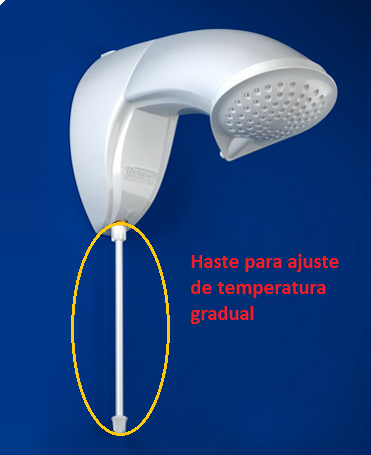
\includegraphics[width=5cm]{imagens/ducha_thermosystem.png}

\label{Ducha ThermoSystem}

\caption{Ducha ThermoSystem}

\end{figure}

O circuito interno da ducha ThermoSystem é bastante simples porém eficiente. Ele é constituído de um potenciômetro, um resistor, dois capacitores em paralelo, um DIAC e um TRIAC. A haste do chuveiro controla o potenciômetro. Este potenciômetro, ao aumentar ou diminuir o valor da resistência, regula o tempo de carga dos capacitores em paralelo. Os capacitores, por sua vez, ao atingirem o valor de tensão de 24V acionam o DIAC que consequentemente acionará o TRIAC. O TRIAC ao ser acionado fecha o circuito, possibilitando a passagem de corrente elétrica pela carga do chuveiro (resistência). Dessa maneira é possível regular o ângulo de disparo de um sinal possibilitando a aplicação de potências diferentes em uma carga. A figura 3.2 representa o circuito interno da ducha ThermoSystem.



\begin{figure}[!htb]

\center

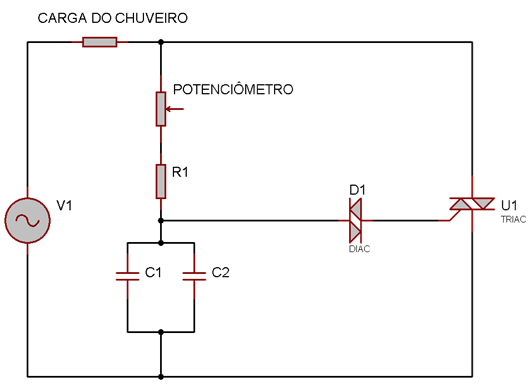
\includegraphics[width=10cm]{imagens/circuito_thermosystem.png}

\label{Circuito interno da ducha ThermoSystem}

\caption{Circuito interno da ducha ThermoSystem}

\end{figure}


\section{Etapas}
Nesta seção serão comentadas as etapas e as implementações realizadas pelo \textit{software} do projeto do regulador de temperaturas. A figura abaixo mostra o fluxograma do \textit{software} utilizado.


\begin{figure}[!htb]

\center

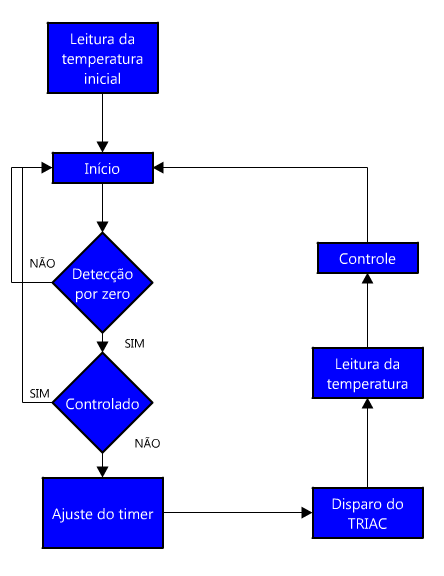
\includegraphics[width=10cm]{imagens/fluxograma_melhor.png}

\label{Fluxograma do software do projeto}

\caption{Fluxograma do software do projeto}

\end{figure}

\subsection{Detecção de passagem por zero}

A detecção de passagem por zero do sinal CA (corrente alternada) foi necessário pois somente dessa forma se teria um controle preciso do ângulo de fase do sistema. A implementação da detecção de passagem por zero foi realizada com o auxílio de um transformador de 6V+6V, um retificador de onda completa, um divisor resistivo e um pino de entrada analógica do microcontrolador ATmega328. O sinal CA da saída do transformador, após ser retificado, passa pelo divisor resistivo implementado para que a tensão seja reduzida de 6V para uma tensão menor que 5V (tensão máxima suportada nas portas do microcontrolador ATmega328). A saída do divisor resistivo é conectada a porta analógica $A_0$ do microcontrolador do qual irá detectar toda vez que o sinal retificado e reduzido passar por zero volt.

\subsection{Leitura da temperatura}
A leitura da temperatura da água se torna necessária, uma vez que o usuário irá entrar com a temperatura desejada do banho e este valor de referência será comparado com a temperatura atual da água. O sensor utilizado para a medição da temperatura da água é o LM35. Este sensor se comporta de forma linear, e fornece uma tensão de 10$\frac{mV}{^\circ C}$ sendo a temperatura máxima medida de 150$^\circ$C, fornecendo assim uma tensão máxima de 1,5V. A tabela 3.1 mostra os pinos do microcontrolador em que o sensor é conectado.

\begin{table}[!hbt] 
   \centering   % tabela centralizada
   \setlength{\arrayrulewidth}{1\arrayrulewidth}
   \setlength{\belowcaptionskip}{5pt}
   
   \caption{Conexões do sensor de temperatura ao Arduino}
   \begin{tabular}{l|l} % c=center, l=left, r=right 
      \hline
      \textbf{Terminal do sensor} & \textbf{Pino do Arduino} \\
      \hline
      Alimentação ($+V_S$) &  5V  \\
      \hline
      Saída analógica ($V_out$)  & A1 \\
      \hline
      Terra (GND)	& GND \\
      \hline
   \end{tabular}
   \label{Conexões do sensor de temperatura ao Arduino}
\end{table}
Um resistor de 2,2k$\Omega$, conectado entre o terra e a saída do sensor, foi utilizado para a redução de ruídos e possíveis erros de medição

O sensor foi configurado para medir temperaturas entre 2$^\circ$C até 110$^\circ$C. Esta configuração foi realizada mudando-se a referência do conversor A/D de 5V (referência padrão) para 1,1V (referência interna do microcontrolador). Desta forma, o conversor A/D irá fornecer um valor de 1023 quando o sensor estiver marcando 110$^\circ$C, diminuindo assim a influência de possíveis ruídos externos em comparação à referência de 5V. Com a referência em 1,1V, para cada aumento de uma unidade na leitura do conversor A/D temos um aumento de $\frac{1,1V}{1024}$, ou seja, 1,07mV.

Para diminuir os efeitos dos ruídos, presentes no sensor LM35, foi feita uma média aritmética de 20 leituras do sensor de temperatura, dessa forma tem-se uma melhor precisão da temperatura medida.

Com a saída do sensor de temperatura conectada a porta analógica $A_1$ do Arduino, utilizou-se a seguinte equação para a conversão de tensão em temperatura:

\begin{center}
Temperatura $ = \frac{1,1}{1024}.100.AD$
\end{center}
\noindent onde a variável Temperatura é dada em $^\circ$C, AD representa a leitura do conversor A/D. O valor 100 é utilizado para transformar o valor de tensão em $^\circ$C.

\section{Controle}
O levantamento da planta do sistema foi realizado utilizando-se o \textit{software} Matlab. 

Primeiramente foi realizada a aquisição de dados do sistema com o auxílio do sensor de temperatura LM35 e o Arduino. O sensor e seus terminais foram envolvidos com espaguete termoretrátil e silicone, para que não houvesse passagem de água na parte interna do sensor, ocasionando erros de medição.A figura 3.4 mostra o sensor com a proteção aplicada.
\begin{figure}[!htb]

\center

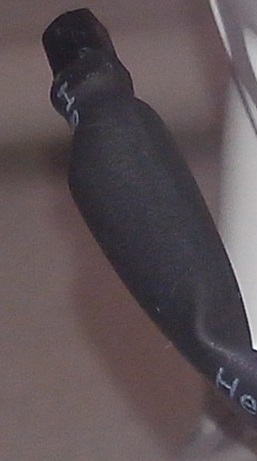
\includegraphics[width=4cm]{imagens/lm35_termoretratil.jpg}

\label{Sensor LM35 com espaguete termoretrátil}

\caption{Sensor LM35 com espaguete termoretrátil}

\end{figure}

\noindent Os terminais do sensor foram soldados nos fios de um cabo de par trançado, mais conhecido como cabo de rede. O motivo da escolha deste cabo foi a sua tolerância a interferências, fácil manuseio e maleabilidade.

Os dados adquiridos foram os de temperatura da água em função do tempo, com o funcionamento do chuveiro em potência máxima, ou seja, a resposta à um degrau de potência. Na figura 3.5 são mostrados os dados adquiridos pelo microcontrolador e plotados com a ferramenta Matlab.

\begin{figure}[!htb]

\center

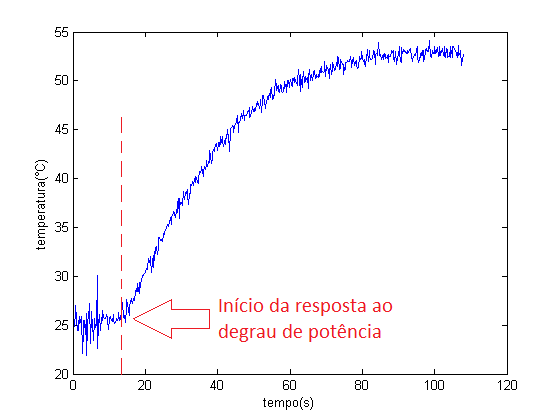
\includegraphics[width=10cm]{imagens/temperatura_por_tempo_reduzido_ambiente.png}

\label{Gráfico Temperatura X Tempo}

\caption{Gráfico Temperatura X Tempo}

\end{figure}

\subsection{Planta do sistema}

\noindent O tempo para o sistema atingir o regime permanente com a potência máxima foi por volta de 85 segundos.
Com os dados adquiridos, uma ferramenta do Matlab chamada \textit{System Identification Toolbox} foi utilizada para a identificação da planta do sistema. Antes de se utilizar essa ferramenta foi necessário deslocar os dados da temperatura para que fossem analisados a partir do zero, ou seja, reduziu-se a temperatura inicial (ambiente), como mostrado na figura 3.6.

\begin{figure}[H]

\center

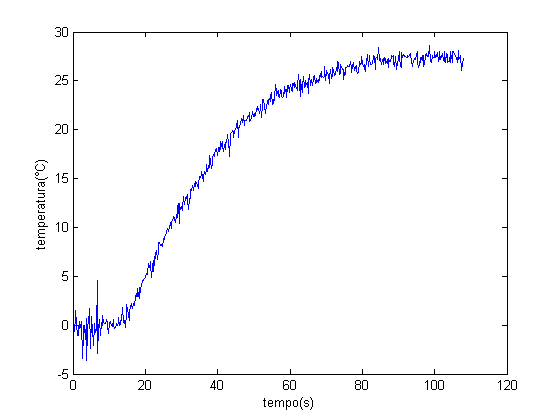
\includegraphics[width=10cm]{imagens/temperatura_tempo_ident.png}

\label{Gráfico Temperatura X Tempo partindo do zero}

\caption{Gráfico Temperatura X Tempo partindo do zero}

\end{figure}

O \textit{System Identification Toolbox} pode ser acessado com o comando "\textit{ident} dentro do ambiente de programação do Matlab. A planta a ser identificada tem como entrada a tensão CA da rede elétrica, que vai ser aplicada a carga do chuveiro (resistência), e como saída a temperatura da água em função do tempo. Os dados adquiridos foram importados para a ferramenta e desta forma a planta do sistema foi identificada com a função de transferência mostrada na equação abaixo.

\begin{center}
$G(s) = \frac{28,524}{25,367s + 1}$

\end{center}

A figura 3.7 faz uma comparação entre a planta obtida e os dados e mostra que a planta adquirida pela ferramenta representa o sistema de forma satisfatória.

\begin{figure}[H]

\center

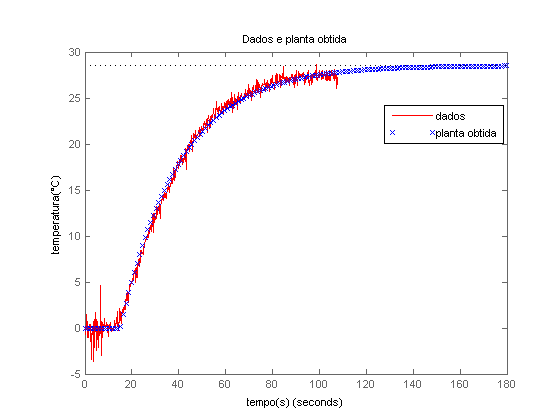
\includegraphics[width=10cm]{imagens/grafico_planta_dados.png}

\label{Comparação entre dados e planta do sistema}

\caption{Comparação entre dados e planta do sistema}


\end{figure}

\subsection{Tempo Morto}

Ao coletar-se os dados de temperatura em função do tempo foi notado que o sensor de temperatura LM35 apresenta um tempo de reposta de cerca de quatro segundos. Devido a este atraso, a planta do sistema foi modificada para a seguinte expressão:

\begin{center}

$G_d(s) = G(s).e^ {-4s}$

\end{center}

\noindent onde $G_d(s)$ representa a planta do sistema agora levando-se em conta o tempo de resposta de quatro segundos ($e^{-4s}$).
Para a eliminação desse tempo morto da malha de controle foi utilizado uma estratégia de controle chamada Preditor de Smith.

\subsection{Controlador}

O controlador utilizado para a implementação do sistema foi o controlador PI (Proporcional Integral). Ele é o conjunto do controlador proporcional e o controlador integral trabalhando em paralelo. Utilizando a ferramenta do Matlab chamada \textit{PID Tuner}, através do comando \textit{pidtool}, foi possível calcular os coeficientes do controlador PI. Os coeficientes do controlador foram calculados para que o sistema tivesse um tempo de resposta de cerca de 12 segundos,para que o tempo até o regime permanente fosse de aproximadamente de 40 segundos e para que não houvesse \textit{overshoot}.

\begin{figure}[H]

\center

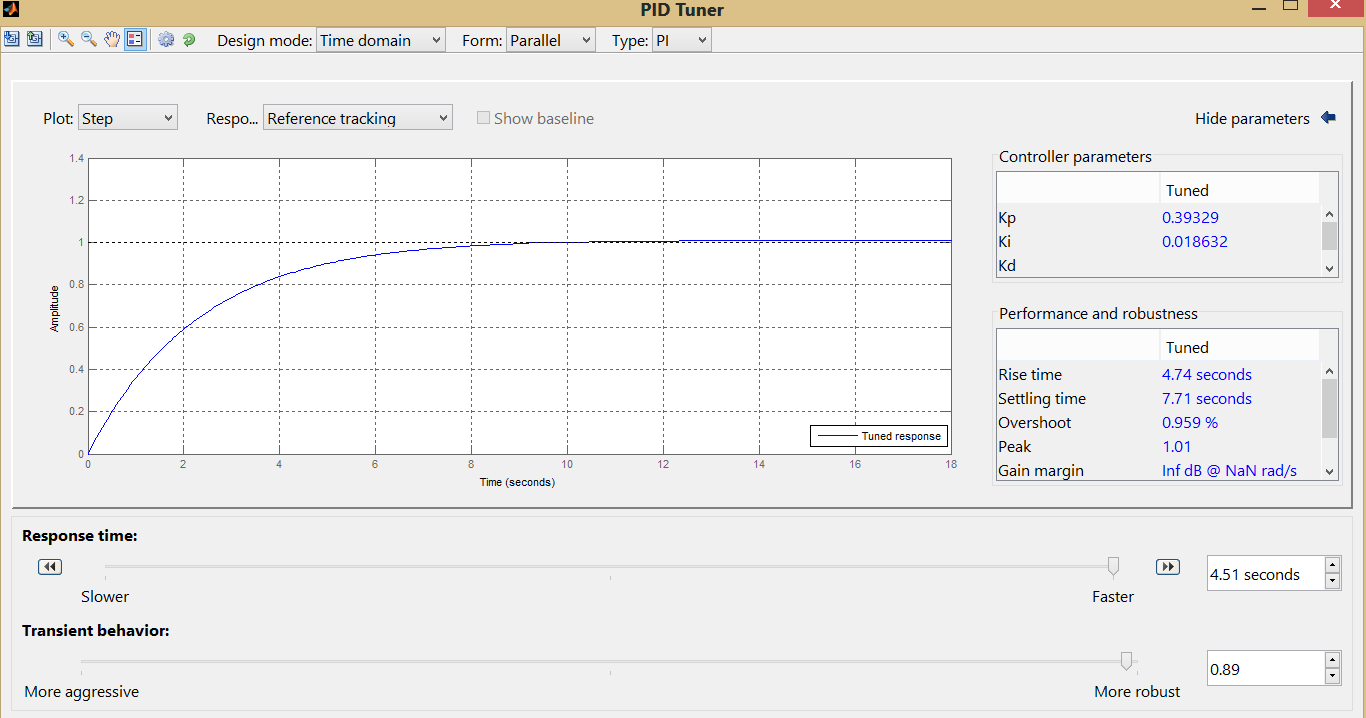
\includegraphics[width=10cm]{imagens/PID_TUNER.png}

\label{PID Tuner}

\caption{PID Tuner}
\end{figure}

Com os coeficientes calculados, a função de transferência é representada na equação a seguir:

\begin{center}

$G_p(s) = \frac{0,143 s + 0,00566}{s}$
\end{center}

    Com a obtenção de todos os parâmetros necessários para a implementação do sistema de controle foi possível representar a malha de controle como mostra a figura 3.9.
    
\begin{figure}[H]

\center

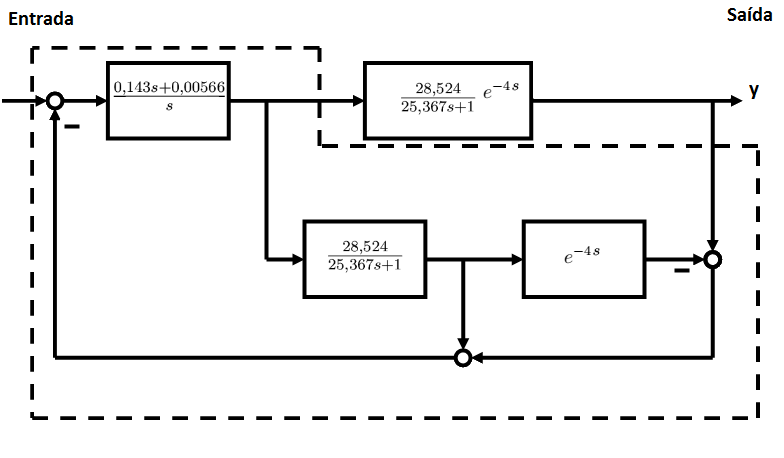
\includegraphics[width=10cm]{imagens/preditor_smith_chuveiro.png}

\label{Malha de controle do regulador}

\caption{Malha de controle do regulador}
\end{figure}
    
    

\subsection{Discretização}

Para a implementação das leis de controle em linguagem de programação para o microcontrolador foi necessário a discretização das funções de transferência uma vez que elas foram obtidas no domínio do tempo contínuo e os microcontroladores trabalham apenas com sinais amostrados, ou seja, no domínio do tempo discreto.

O \textit{software} Matlab possui uma função chamada \textit{c2d(sys,Ts)}, que realiza essa conversão. Os parâmetros \textit{sys}  e \textit{Ts} representam respectivamente a função de transferência a ser discretizada e o tempo de amostragem. O tempo de amostragem empregado neste projeto é de um segundo, que é o intervalo de tempo de coleta do dado de temperatura da água.

Com os parâmetros obtidos, foi possível realizar a conversão para o domínio do tempo discreto como mostra a tabela 3.2.


\begin{table}[!hbt] 
   \centering   % tabela centralizada
   \setlength{\arrayrulewidth}{1\arrayrulewidth}
   \setlength{\belowcaptionskip}{5pt}
   
   \renewcommand{\arraystretch}{2}
   
   \caption{Discretização do sistema contínuo}
   \begin{tabular}{|l|l|l|} % c=center, l=left, r=right 
      \hline
      \textbf{Função} &\textbf{Sistema contínuo} & \textbf{Sistema discreto} \\
      \hline 
      Controlador & $G_p(s) = \frac{0,143 s + 0,00566}{s}$ &  $G_p(z) = \frac{0,143z-0,1374}{z-1}$ \\ 
     \hline
     
     
      Planta do sistema & $G(s) = \frac{28,52}{25,37s+1}$  & $G(z) = \frac{1,103}{z - 0,9613}$ \\
      
      
      \hline 
      Planta do sistema com atraso &$G_{at}(s) = \frac{28,52}{25,37s+1}.e^{-4s}$ & $G_{at}(z) = \frac{1,103}{z - 0,9613}.z^{-4}$ \\  
      \hline 
   \end{tabular}
   \label{Discretização do sistema contínuo}
\end{table}

\section{Ajuste do timer e disparo do TRIAC}

Para controlar o ângulo de disparo do TRIAC foi utilizado o recurso de interrupção por tempo do microcontrolador.

A corrente alternada ao passar pelo retificador de onda completa tem, na saída, uma onda com frequência e período modificados. Como a tensão presente nas residências possui uma frequência de 60Hz, ao ser retificada ela passa a ter a frequência de 120Hz. A figura 3.10 mostra como funciona a retificação do sinal.

\begin{figure}[H]

\center

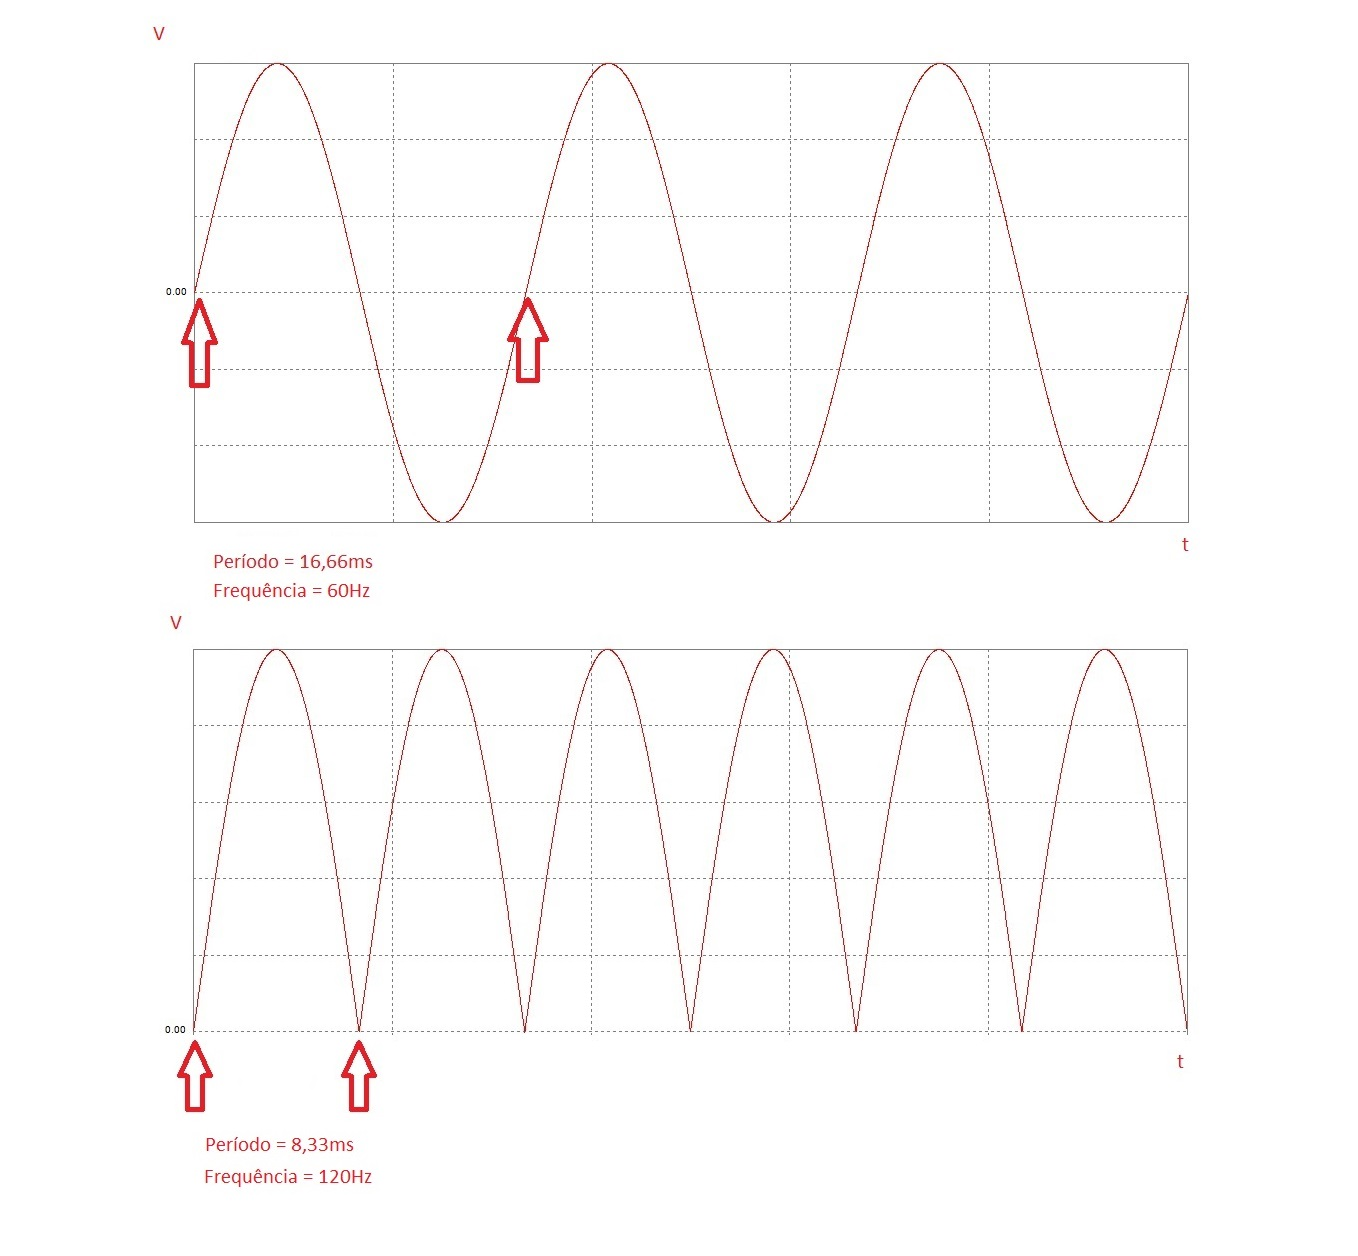
\includegraphics[width=12cm]{imagens/retificacao_sinal.jpg}

\label{Sinal retificado}

\caption{Sinal retificado}
\end{figure}


Como pode-se observar, o período da onda passa de 16,66ms para 8,33ms. Dessa forma, o disparo do TRIAC deverá ser executado no intervalo de tempo calculado pela equação a seguir:

\begin{center}
$t = (1-d).8,33$
\end{center}
\noindent onde d é o \textit{duty cycle} (valor entre 0 e 1), obtido na saída do controlador PI do sistema, e $t$ é o intervalo de tempo, em milissegundos, em que a interrupção deverá ser executada. 

A interrupção por tempo gerada pelo microcontrolador executa uma rotina da qual tem a função de gerar um pulso de 5V, procedente de um pino digital, para o optoacoplador MOC3020. O pulso gerado liga o \textit{led} interno do optoacoplador que, por sua vez, aciona o fotodiac do componente permitindo a passagem de corrente elétrica nos terminais 4 e 6, responsáveis pelo disparo do TRIAC. Um exemplo de controle de disparo pode ser visto na figura 3.11 a seguir.

\begin{figure}[H]

\center

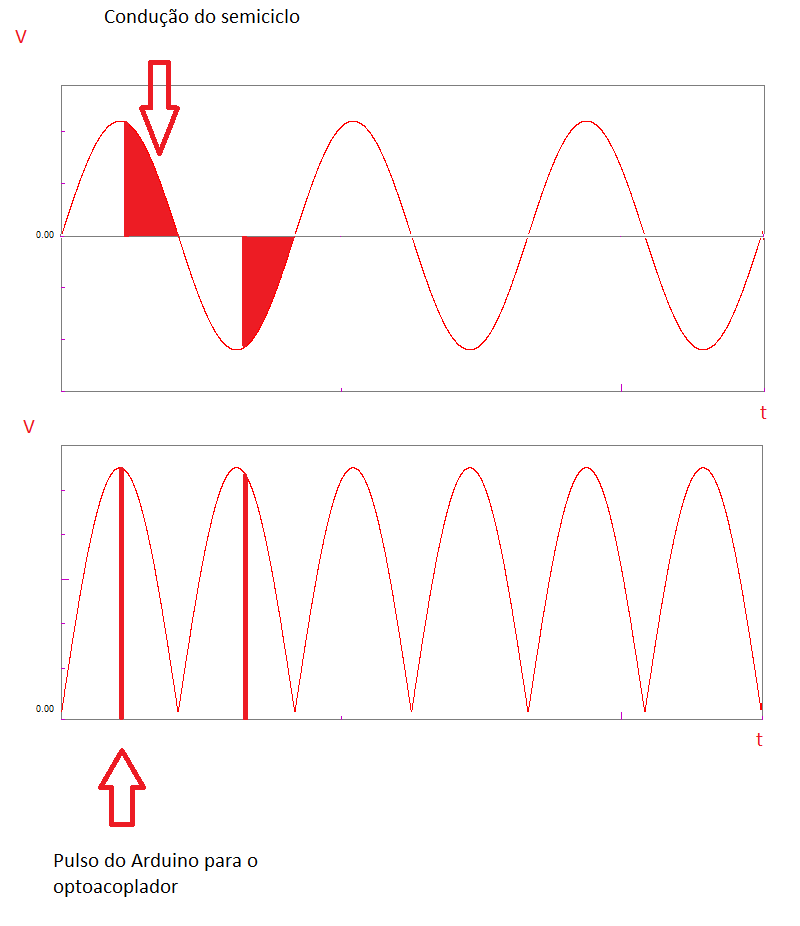
\includegraphics[width=10cm]{imagens/pulso_arduino.png}

\label{Exemplo de controle de ângulo de condução}

\caption{Exemplo de controle de ângulo de condução}
\end{figure}

